\documentclass[9pt]{extarticle}

\usepackage{blindtext}

% Citations as footnotes
% \usepackage[style=verbose,backend=bibtex]{biblatex}
% \bibliography{refs.bib}

\usepackage{amsmath}
\usepackage{amssymb}
\usepackage{graphicx}
\usepackage{microtype}

% Directory for images
\graphicspath{{images/}}

% To wrap text around figures
\usepackage{wrapfig}

% Define new type of columns
\usepackage{array}
\usepackage{tabulary}
\newcolumntype{K}[1]{>{\centering\arraybackslash}m{#1}}

% Stretch the dimension of the rows in tables
\renewcommand{\arraystretch}{1.6}

% Add colors to table
\usepackage{colortbl}

% Set Helvetica as main font
\usepackage{helvet}
\renewcommand\familydefault{\sfdefault}
\usepackage[T1]{fontenc}

% Set Helvetica as main font for equations
\usepackage[helvet]{sfmath}

% Set Helvetica as main font for equations (alternative)
% \usepackage{eulervm}

% Change geometry of the page
\usepackage[left=2cm,top=2cm,right=1.5cm,bottom=1.5cm]{geometry}

% Change spacing
\usepackage{setspace}
\onehalfspacing

\usepackage[svgnames]{xcolor}
\usepackage[pdftex]{hyperref}
\hypersetup{colorlinks=true,linkcolor=blue,citecolor=ForestGreen,urlcolor=DarkOrchid}

% Where images are located
\graphicspath{{images/}}

% Redefine names
\newcommand{\sectionname}{Section}
\renewcommand{\appendixname}{Appendix}
\newcommand{\equationname}{Equation}
\newcommand{\referencename}{Ref.}
\renewcommand{\figurename}{Figure}
\renewcommand{\tablename}{Table}

% Adjust section titles
\usepackage{titlesec}
\titleformat{\section}{\bfseries\normalsize}{\thesection.}{0.5em}{}

% Change position of the page number
\usepackage{fancyhdr}
\pagestyle{fancy}
\renewcommand{\headrulewidth}{0pt}
\fancyhf{}
\fancyhead[R]{\thepage}

% Add notes to the text
\usepackage{changes}
\newcommand{\note}[1][]{\added[remark={#1}]}

% Some useful definition
\newcommand{\DW}{\mbox{D-Wave 2X\textsuperscript{TM}}~}

\begin{document}

\begin{center}\Large
\textbf{Exploration of the Potential of Quantum Annealing for Hard Scheduling
Problems in Air Traffic Management: Report, July 2016}
\end{center}

\def\changemargin#1#2{\list{}{\rightmargin#2\leftmargin#1}\item[]}
\let\endchangemargin=\endlist 

\section*{Introduction}\label{sec:intro}

Given encouraging of early results in the planning domain \cite{rieffel:15,venturelli:15}
and the expertise of our team in such sector, 
aim of the project is to use Quantum Annealing (QA), and in particular the state-of-art \DW quantum annealer hosted at NASA Ames, 
as a metaheuristic for solving computational challenging problems in the context of
Air Traffic Management (ATM). More precisely, the project has been focused on the problem to find distinct minimum-cost configuration scheduling advisories (CSAs).
In this project, we limit our attention to the North Atlantic oceanic airspace (NAT) for which we have optimal-wind trajectories
for two consecutive days (July 28\textsuperscript{th}-29\textsuperscript{th} 2012).

Since the \DW quantum chip can only optimize binary optimization problems on a specific and fix-by-design architecture called Chimera,
in the first part of the project we mainly focused on the formulation of CSAs in terms of discrete variables (\tablename~\ref{table:milestone} for tasks/milestones
of the project). The discrete model is then expressed in terms of quadratic binary optimization (QUBO) problems that can be natively solved by 
the \DW quantum chip. The next set of milestones will include the run of CSA instances on the \DW quantum chip, as well as the comparison of the results
with the best state-of-art classical QUBO optimizers.

\section*{Approach and technical details}\label{sec:approach}

%
\begin{wrapfigure}{r}{0.38\textwidth}
\centering
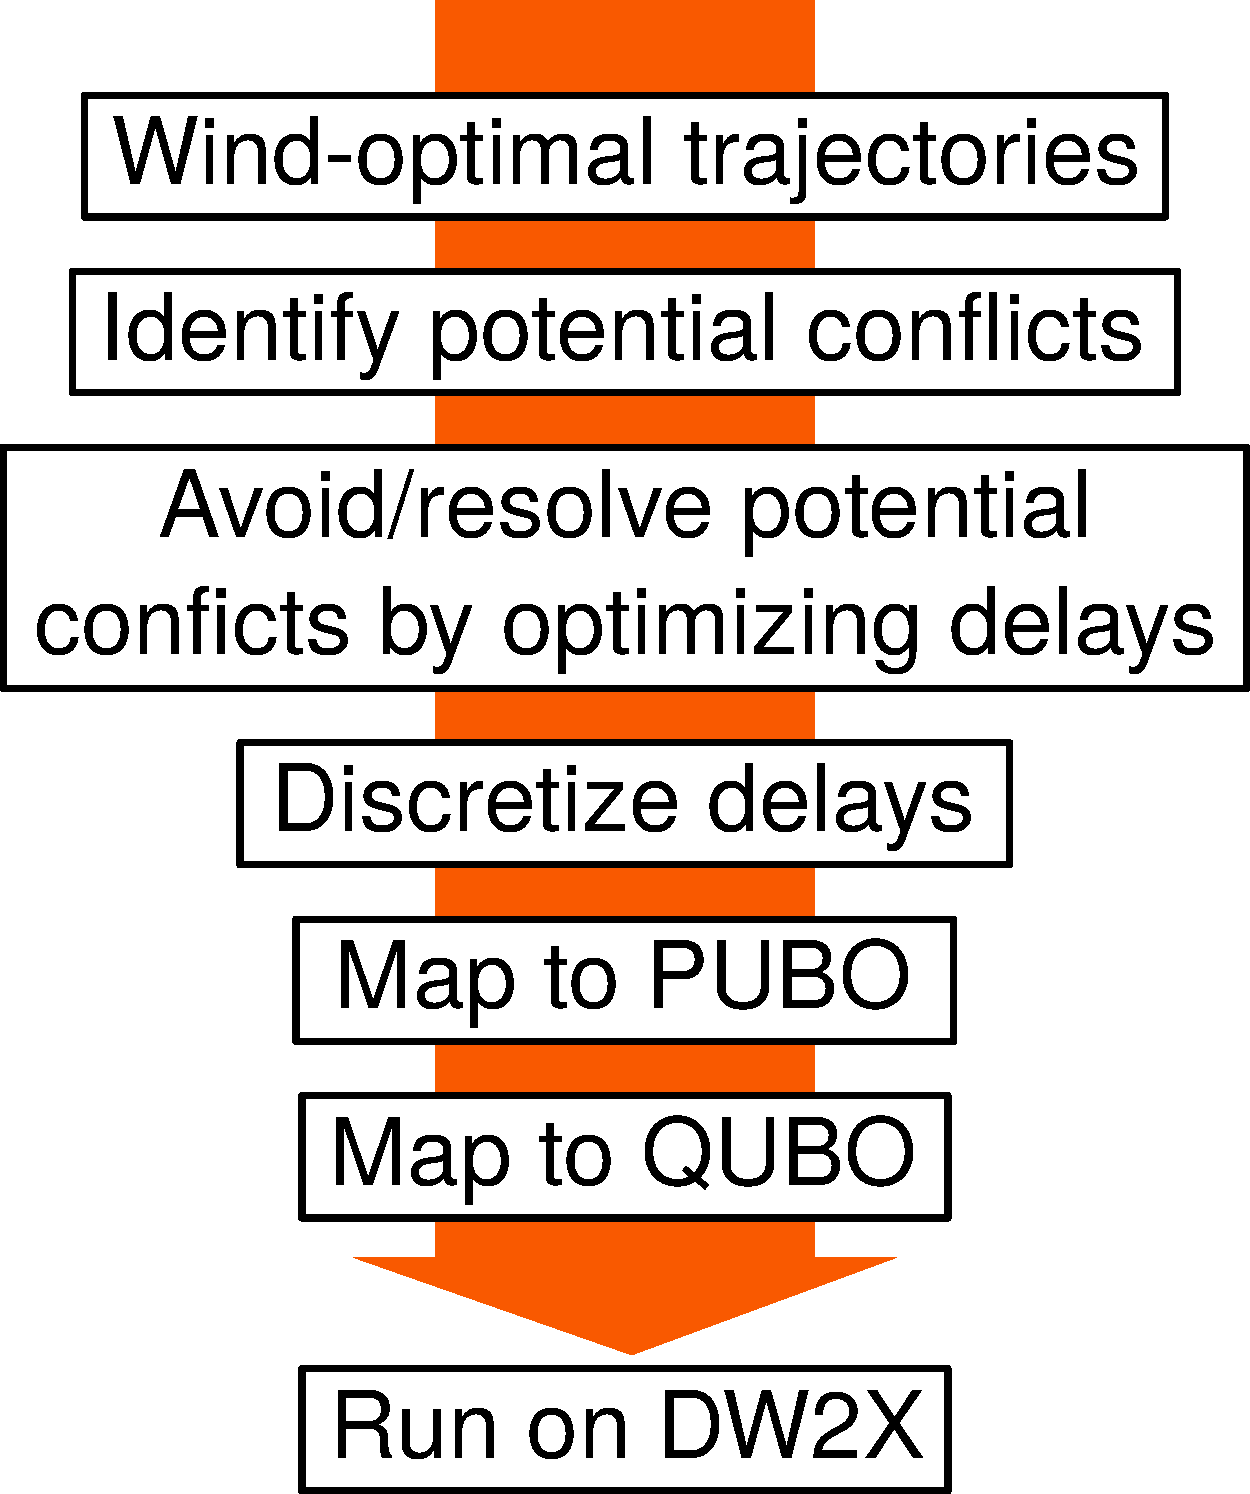
\includegraphics[width=0.25\textwidth]{scheme}
\caption{\label{fig:scheme}Flow diagram to map ATM problems onto the \DW quantum chip.}
\end{wrapfigure}
%
NAT dataset consists in \note[What is the number of trajectories?]{XXX} wind-optimal trajectories in (3+1)-dimensions. Since wind-optimal
trajectories have been computed independently from each others, two or more trajectories can intersect in space creating a ``conflict''. 
A conflict becomes ``potential'' if two or more flights can reach at the \emph{same} time the spatial conflict. CSAs consist
in finding minimal changes of the wind-optimal trajectories to avoid all the potential conflicts. 
Given the fixed architecture and the limited amount of physical resources of the \DW quantum chip, it is impossible to directly CSAs problems
on on the quantum hardware. For this reason, a series of transformation of the original CSA formulation must be performed before 
to use the quantum chip as optimizer. \figurename~\ref{fig:scheme} summarizes the transformation we used in this project:

\begin{changemargin}{0.5cm}{0cm}
\textbullet~\textbf{Identify potential conflict.} In principle, any conflict is a potential conflict: indeed, flights can accumulate delay
and therefore arrive at the same to a spatial conflict. Nevertheless, the number of spatial conflicts is prohibitive. To limit the number
of potential conflicts, we pre-processed the wind-optimal trajectories assuming a \emph{time} delay of at most \note[Check this]{$1$ hour} and
eliminating all the potential conflict that do not respect the bound. This process reduce the number of potential conflicts from
\note[Please add some numbers.]{XXX to XXX}.
\end{changemargin}

\begin{changemargin}{0.5cm}{0.5cm}
\textbullet~\textbf{Avoid/resolve potential conflicts by optimizing delays.} Even after the reduction of potential conflicts, it would be impossible to directly
map the (3+1)-dimensional trajectories onto the \DW quantum chip. Instead, we formulate the CSAs in terms of a ``delay'' problem. More precisely,
let us define the time $T_{ik}$ of a flight $i$ to reach a potential conflict $k$, that is:
\begin{equation}\label{eq:T}
	T_{ik}(d_i,\,\left\{d_{ip}\right\}) = t_{ik} + d_i + \sum_{p\in \mathcal{P}^{<k}_i} d_{ip},
\end{equation}
with $t_{ik}$ the wind-optimal time to reach the conflict $k$, $d_i$ the delay at the departure, 
$\mathcal{P}^{<k}_{i}$ the set of potential conflicts $p$ that antecede the conflict $k$ and $d_{ip}$ the delay
of flight $i$ at the potential conflict $p$. In the above formulation, it is assumed that all the maneuvers to avoid potential conflicts
consist in small and local changes of the wind-optimal trajectories that do not create a cascade of new potential conflicts and do not
change the location of the existing potential conflict. The cost function to minimize can be then expressed as
\begin{equation}\label{eq:f}
	f(\left\{d_i\right\},\,\left\{d_{ip}\right\})= \sum_{i} d_i + \sum_{ip} d_{ip},
\end{equation}
where all the $\left\{d_i\right\}$ and $\left\{d_{ip}\right\}$ are constrained so that two flights $i$ ($j$) have a different arrival time
$T_{ik}$ ($T_{jk}$) to the same potential conflict $k$, namely
\begin{equation}\label{eq:theta}
	\Theta_{a_{ijk}}(\left|T_{ik} - T_{jk}\right|) = 0,
\end{equation}
with $\Theta$ a certain function which ensure that the two flights are far apart to complete their maneuvers. Here, $a_{ijk}$ represent
some extra-parameters that can be added to the model to have more control on the maneuvers.
\end{changemargin}

\begin{table}[t!]\centering
	\begin{tabular}{|m{7cm}|m{7cm}|K{1.8cm}|}
		\rowcolor{gray!30}
		\hline
		\multicolumn{1}{|c|}{\textbf{Task/Milestone}} & \multicolumn{1}{c|}{\textbf{Performance Metric}} & \textbf{Expected completion}\\
		\hline
			Map the ATM problem to a suitable polynomial binary optimization problem (PUBO). & 
				Number of required qubits. Largest degree of the polynomial. Connectivity of the underlying coupling graph. & \checkmark\\
		\hline
			Map the ATM problem to a suitable quadratic binary optimization problem (QUBO). &
				Number of required qubits. Connectiviry of the underlying coupling graph. & \checkmark\\
		\hline
			Identify a set of benchmark ATM problems. & Hardness as a function of size. & 1 month\\
		\hline
			Analyze the results/performance of classical QUBO solvers on ATM problems. & 
				Assess the quality/variety of the solutions after discretization. Find the bottom line for classical computation. & 1.5 month\\
		\hline
			Find an embedding to map the ATM problem onto the Chimera architecture. & 
				Overhead of the embedding. Largest ATM problem embeddable on the current \DW chip. & 2 month\\
		\hline
			Compile the ATM benchmark ensemble for the \DW chip. & 
				Scaling of expected time to solution vs. size compared to classical code. Variety of different acceptable solutions. & 3 month\\
		\hline
			Outlook on different architectures and annealing strategies, hardware changes &
				Potential quantum enhancement. & 4 month\\
		\hline
	\end{tabular}\caption{\label{table:milestone}Breakdown of the project effort into milestones, including suggested performance metric and completion
		dates (check marks indicate completed tasks).}
\end{table}

\begin{changemargin}{0.5cm}{0.5cm}
\textbullet~\textbf{Discretize delays.} The delay model is completely defined by the \equationname{s}~(\ref{eq:T})-(\ref{eq:theta}). The successive step
consists in the discretization of the variables involved in the delay model. The discretization is achieved by expressing each variable $x$ in terms 
of a discrete set of values $\left\{x_\alpha\right\}$
\begin{equation}\label{eq:discr}
	x = \sum_{\alpha} x_{\alpha}\sigma_\alpha,
\end{equation}
with $\sigma_{\alpha} = \{0,\,1\}$, and then enforcing that only one among all the $\left\{\sigma_\alpha\right\}$ is one, namely
\begin{equation}\label{eq:constr}
	\sum_\alpha \sigma_\alpha = 1.
\end{equation}
\end{changemargin}

\begin{changemargin}{0.5cm}{0.5cm}
\textbullet~\textbf{Map to PUBO.} Using the discretization in \equationname~(\ref{eq:discr}), with the constraint given by \equationname~(\ref{eq:constr}), the cost function
$f$ in \equationname~(\ref{eq:f}) of the delay model can be therefore expressed as a polynomial unconstrained binary optimization (PUBO).
\end{changemargin}

\begin{changemargin}{0.5cm}{0.5cm}
\textbullet~\textbf{Map to QUBO.} The \DW quantum chip can only natively solve quadratic unconstrained binary optimization (QUBO) problems. Therefore, a reduction 
from a PUBO, which involves higher order polynomials, to QUBO is necessary. The reduction can be done using two different approaches. On one hand, it is possible to
use gadgets to reduce higher order polynomials to quadratic terms \cite{babbush:13}. On the other hand, one can use Lagrange multipliers \cite{ronagh:15} 
to enforce constraints as in \equationname~(\ref{eq:constr}) and then reduce the number of higher order polynomials.
\end{changemargin}

\section*{Assessment and conclusions}\label{sec:ass}

We have devised the delay model to reduce ATM problems to QUBO problems, which are natively solved by the \DW quantum chip. Despite its simplicity,
the model can still capture many of the properties of ATM problems. Next step of the project will be to analyze the quality/variety of the solutions
of the delay model using state-of-art classical QUBO optimizers. This will give us a bottom line for the performance of quantum annealers. Finally,
we will run the ATM problems on the current \DW quantum chip and compare the quality of results with the classical counterpart. Given the limited
amount of resources for the \DW quantum chip, we will benchmark the quantum annealer using small problems. The potential quantum enhancement will
be then extrapolate from the data. See \tablename~\ref{table:milestone} for a complete overview of tasks/milestones.

\bibliographystyle{unsrt}
\bibliography{refs.bib}

\end{document}
